\chapter{Controller Theory}
\label{ch:chapter_four}%
% The \label{...}% enables to remove the small indentation that is generated, always leave the % symbol.

\section{E-Cargo System}
\label{sec:E-Cargo}

As introduced in the first chapters, the object of this thesis is a Smart Electric Cargo (Figure \ref{fig:E-Cargo CAD drawing}).


\begin{figure}
    \centering
    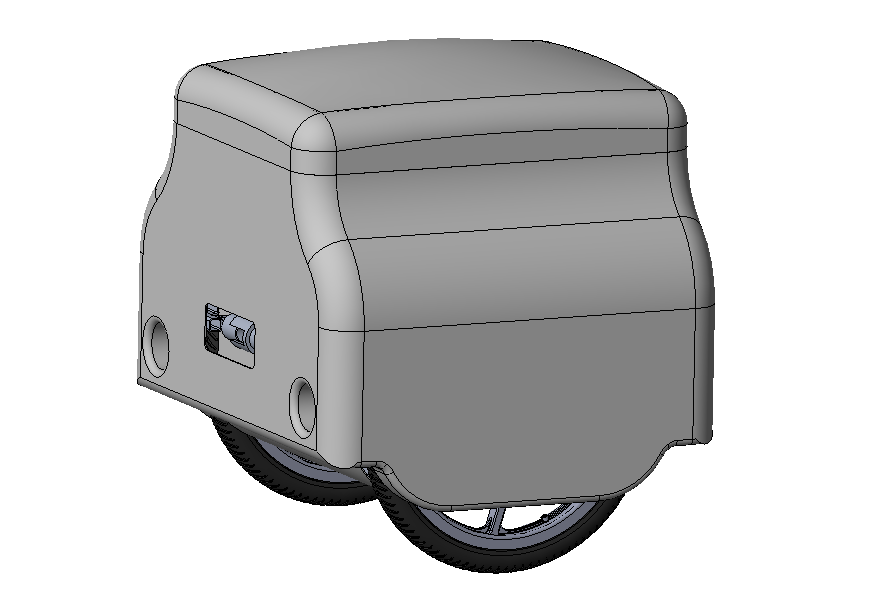
\includegraphics[width=0.5\linewidth]{e-Cargo CAD.png}
    \caption{E-Cargo CAD drawing.}
    \label{fig:E-Cargo CAD drawing}
\end{figure}

The mechanical design has been realized, taking into account that the Center of Mass must always lye above the wheels' axle and so all the electronic devices (sensors, computers, battery...) are placed accordingly.
This design makes the E-Cargo a TWIP also for the unloaded configuration.

The motion is given by two in-wheeled electric motors (BLDC), and two small safety wheels (not represented in the CAD) have been mounted on both sides to guarantee an initial starting pitch angle of $\approx 25^{\circ}$.
Table \ref{tab:E-Cargo Mechanical Parameters} provides a summary of all the key parameters relevant to the controller simulation, which can help in better understanding the results.
The numbers are qualitative since the mechanical/design concept is still evolving:

\begin{table}[H]
    \centering
    \renewcommand{\arraystretch}{1.5} % Increase the vertical spacing between rows
    \begin{tabular}{@{}l@{\hspace{1.5cm}}l@{\hspace{1.5cm}}l@{\hspace{1.5cm}}l@{\hspace{1.5cm}}l@{}}
    \toprule
    \textbf{Symbol} & \textbf{Description} & \textbf{Units} & \textbf{Value} & \textbf{Notes} \\
    \midrule
    $m$ & Mass of the cargo & $kg$ & 20 & mass unloaded \\
    $m_{p}$ & Mass of payload & $kg$ & 40 & maximum payload \\
    $I_y$ & Y Moment of inertia & $kg m^2$ & 3.3 & pitch moment of Inertia  \\
    $I_z$ & Z Moment of inertia & $kg m^2$ & 2.4 & yaw moment of inertia \\
    $r_w$ & Wheel radius & $m$ & 0.2 & wheel radius \\
    $CoM_{z}$ & CoM height & $m$ & 0.3 & Max CoM height w.r.t wheels' axle \\
    $b$ & axle length & $m$ & 0.6 & length of the wheels' axle \\
    $h$ & height & $m$ & 0.9 & total height \\
    $l$ & length & $m$ & 0.5 & total length \\
    $w$ & width & $m$ & 0.6 & total width \\
    \bottomrule
    \end{tabular}
    \caption{E-Cargo Mechanical Parameters.}
    \label{tab:E-Cargo Mechanical Parameters}
\end{table}


\section{E-Cargo Dynamical Model}
\label{sec:E-Cargo Dynamical model}

In \cref{ch:chapter_three} we have described the basic architecture of the control framework; in this chapter, we will follow the same approach, adapting each case specifically to our robot.
Starting from the EoM written for a generic floating base system:

    \begin{equation*}
          M(\mathbf{q})\dot{\bm{\nu}} + C(\mathbf{q},\bm{\nu})\bm{\nu} + \mathbf{g}(\mathbf{q}) = S\bm{\tau} + \sum_{k \in \mathcal{I}_C} J^{T}_{k}\mathbf{f}_{k},
    \end{equation*}

there are two main aspects that require more details:

    \begin{itemize}
        \item The Contact wrench $\mathbf{f}_{k}$.
        \item The Contact Jacobian $J_{k}$.
    \end{itemize}

\subsection{Contact Wrench}
\label{subsec:Contact Wrench}

A first definition for the contact wrench representing the total forces acting on a rigid body has been provided in \cref{sec:Force-Torque covectors}.
It has been described as a vector 

\begin{equation}
    {}_{B}\mathbf{f} = 
    \begin{Bmatrix}
    {}_{B}\bm{f} \\
    {}_{B}\bm{\mu}
    \end{Bmatrix} \in \mathbb{R}^{6}
\end{equation}

with dimension 6.
The actual dimension of the wrench depends on the assumption that we make on the "\textit{dimension}" of the contact.
For legged robots, the contact is usually assumed to be a surface (the bottom surface of the foot); a force reduction is performed to end up with a point contact, and if this point is a generic one on the surface, this reduction leads to 3 linear components (forces) and 3 angular components (moments)(Figure\ref{fig:6DContact_Wrench}).


\begin{figure}
    \centering
    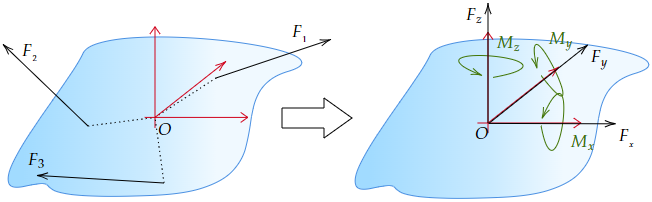
\includegraphics[width=0.65\linewidth]{6DContact_Wrench.png}
    \caption{6D Contact Wrench.}
    \label{fig:6DContact_Wrench}
\end{figure}

In our study, we opted for the following contact modeling assumptions:

\begin{itemize}
    \item Rigid contact model;
    \item Wheels modeled as unidimensional disks;
\end{itemize}

\begin{figure}[H]
    \centering
    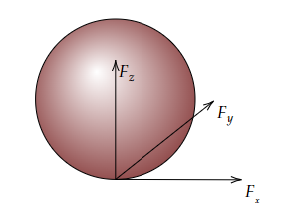
\includegraphics[width=0.35\linewidth]{3DContact_Wrench.png}
    \caption{3D Contact Wrench.}
    \label{fig:3DContact_Wrench}
\end{figure}

These two assumptions result in a final 3D contact wrench, as illustrated in Figure \ref{fig:3DContact_Wrench}. This follows from the fact that the rigid contact between a disk and a plane is inherently a point contact defined by the nature of the interaction and not resulting from a reduction of forces; this is the reason why the angular components are not involved.
The wrench becomes defined as

\begin{equation}
    {}_{B}\mathbf{f} = 
    \begin{Bmatrix}
    {}_{B}\bm{f} \\
    \end{Bmatrix} = 
    \begin{Bmatrix}
    {}_{B}{f}_{x} \\
    {}_{B}{f}_{y} \\
    {}_{B}{f}_{z} 
    \end{Bmatrix} \in \mathbb{R}^{3}.
    \label{eq:3DContact_Wrench}
\end{equation}

Considering that there are two wheels, the total number of contact forces involved is six. The combined contact wrench, derived from the stacking of the two individual wrenches, will be defined as follows:

\begin{equation}
    {}_{B}\mathbf{f}= \sum_{k \in \mathcal{I}_C} {}_{B}\mathbf{f}_{k} = \begin{Bmatrix}
    {}_{B}\bm{f}_l \\
    {}_{B}\bm{f}_r
    \end{Bmatrix} \in \mathbb{R}^{6},
    \label{eq:Total Contact Wrench}
\end{equation}

where ${}_{B}\bm{f}_l$ denotes the contact wrench that acts on the left wheel and ${}_{B}\bm{f}_r$ denotes the contact wrench acting on the right wheel.

\subsection{Rolling Contact Jacobian}
\label{subsec:Rolling Contact Jacobian}

The concept of the contact Jacobian has been introduced in \cref{subsec: Geometric Jacobians}, together with the most complete notation
    \begin{equation*}
        {}^{C_i} J_{A,L/X}(\mathbf{q}) = {}^{C_i}X_{L} {}^{L}J_{A,L/X}(\mathbf{q}).
    \end{equation*}
With reference to Equation \eqref{eq: General contact Jacobian} what has to be higlighted is that, considering a generic link $L$, experiencing the contact $C_i$, in general:
$${}^{C_i} J_{A,L/X}(\mathbf{q}) \neq {}^{C_i}J_{A,C_i/X}(\mathbf{q}),$$
because the frame $C_i$ that is experiencing the contact at a given time instant, can move with respect to the link $L$ and this exactly what happens in the case of a rolling contact.

\begin{figure}
    \centering
    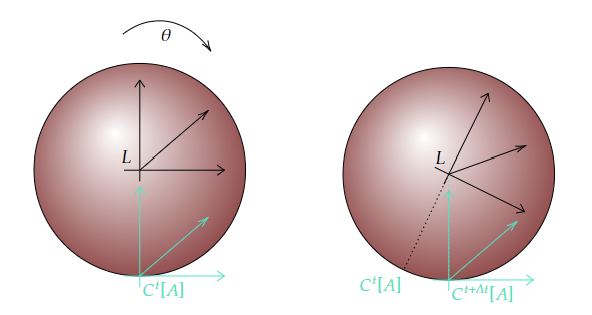
\includegraphics[width=0.5\linewidth]{Rolling_Contact.png}
    \caption{Rolling contact.}
    \label{fig:Rolling contact}
\end{figure}


So in simple words what is usually done is computing the Jacobian of the link's reference frame, and then shifting it to the contact point through a properly defined transformation $X$.


Since we decided to express all in \textit{mixed} representation, the contact Jacobian can be defined as:

    \begin{equation}
        {}^{C_i[A]} J_{A,L/B[A]}(\mathbf{q}) = {}^{C_i[A]}X_{L[A]} {}^{L[A]}J_{A,L/B[A]}(\mathbf{q}),
    \end{equation}
    
where ${}^{L[A]}J_{A,L/B[A]}$ is the \textit{doubly mixed} Jacobian of the wheel calculated in its CoM, and ${}^{C_i[A]}X_{L[A]}$ is a matrix defined as:

\begin{equation}
{}^{C[A]}  X_{L[A]} = \begin{bmatrix} 
{}^{C[A]}  R_{[A]} &    {}^{C[A]} o^\wedge_{L[A]}  {}^{C[A]} R_{L[A]} \\
0_{3x3} & {}^{C[A]} R_{L[A]}\\  
\end{bmatrix}
\end{equation}

that for this specific application, and considering the terrain flat, is just:

\begin{equation}
{}^{C[A]}  X_{L[A]} = \begin{bmatrix} 
I_{3 \times 3} &    {}^{C[A]} o^\wedge_{L[A]} I_{3 \times 3} \\
0_{3x3} & I_{3 \times 3}\\  
\end{bmatrix}.
\end{equation}

Equation \eqref{eq:doubly mixed Jacobian definition} allows us to compute the contact forces even if the contact point changes due to the rolling motion.

From now on, to simplify the notation we will denote ${}^{C_i[A]} J_{A,L/B[A]}(\mathbf{q})$ as $J_{C_{L}}$ for the left wheel and $J_{C_{R}}$ for the right wheel.

For a more compact notation we can stack the Jacobians together (as we did for the wrenches) obtaining the \textbf{overall contact Jacobian} defined as

\begin{equation}
    J_{C} = \begin{bmatrix}
    S_{J_{C}}J_{C_{L}} \\
    S_{J_{C}}J_{C_{R}}
\end{bmatrix} \in \mathbb{R}^{6 \times 8},
\label{eq:overall contact Jacobian}
\end{equation}

where $S_{J_{C}}$ is a selection matrix defined as

\begin{equation}
    S_{J_{C}} = \begin{bmatrix}
        1 & 0 & 0 & 0 & 0 & 0 \\
        0 & 1 & 0 & 0 & 0 & 0 \\
        0 & 0 & 1 & 0 & 0 & 0 \\
    \end{bmatrix}.
\end{equation}

Considering that the input vector $\bm{\tau}$ contains the two torques acting on the left and on the right wheel, respectively, as

\begin{equation}
    \bm{\tau} = \begin{Bmatrix}
    \tau_{L} \\
    \tau_{R}    
\end{Bmatrix} \in \mathbb{R}^{2}.
\end{equation}

The final expression of the robot dynamic equation is given as

\begin{equation}
      M(\mathbf{q})\dot{\bm{\nu}} + C(\mathbf{q},\bm{\nu})\bm{\nu} + \mathbf{g}(\mathbf{q}) = S\bm{\tau} + J_{C} {}_{B}\mathbf{f}.
      \label{eq:e-Cargo dynamic equation}
\end{equation}

\section{Tasks definition}
\label{sec:Tasks definition}

The task definition depends on the specific actions that we want our robot to perform.
In our case, the concept is still evolving, but generally, it requires autonomous navigation and self-balancing:

\begin{itemize}
    \item By \textbf{self-balancing}, we mean that the E-Cargo, given is TWIP configuration, must not fall down.
    \item By \textbf{Tracking}, we mean that the E-Cargo must be able to follow a person or a given signal, requiring as a consequence a control in position.
\end{itemize}

In \cref{ch:chapter_three} we have seen how tasks and constraints have a similar formulation, and this allows to interchange them when needed.

As a starting point we consider them both as tasks, and we will see how to deal with both, starting from the first one.

From this section on, the part of the E-Cargo including the body and payload (i.e., everything above the wheels' axle) is referred to as the "upper assembly" and will be modeled as a single rigid body called \textit{base} $B$.

\subsection{Self-Balancing Task}
\label{subsec:Self-Balancing Task}

The Self-Balancing is the robot's most important feature because, without it, none of the other tasks can be reliably performed.

\begin{figure}
    \centering
    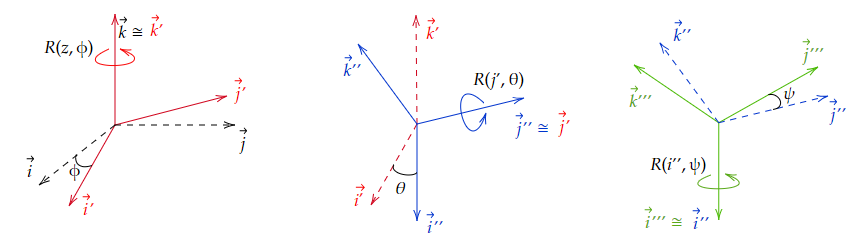
\includegraphics[width=0.9\linewidth]{RPY.png}
    \caption{Yaw-Roll-Pitch decomposition.}
    \label{fig:Yaw-Roll-Pitch decomposition}
\end{figure}

To ensure this, according to Figure \ref{fig:Yaw-Roll-Pitch decomposition} we choose to control the pitch angle of the body named $\theta$.

In the body reference frame, the base angular velocity ${}^{B} \omega_{A,B}$ can be obtained as

\begin{equation}
    {}^{B} \bm{\omega}_{A,B} = \dot{\phi}\,{}^{B}\vec{k} + \dot{\theta}\,{}^{B}\vec{j}' + \dot{\psi}\,{}^{B}\vec{i}''.
    \label{eq:Base_ang_Vel}
\end{equation}

We want to pass to the mixed representation in which we need the right-trivialized base angular velocity ${}^{A} \bm{\omega}_{A,B}$, and to do so we project the geometric vectors involved, in the proper inertial frame defined by:

\begin{equation*}
    {}^{A}\vec{i} = \begin{Bmatrix}
        1 \\
        0 \\
        0
    \end{Bmatrix} ;     {}^{A}\vec{j} = \begin{Bmatrix}
        0 \\
        1 \\
        0
    \end{Bmatrix} ; {}^{A}\vec{k} = \begin{Bmatrix}
        0 \\
        0 \\
        1
    \end{Bmatrix};
\end{equation*}

meaning that 

\begin{equation}
    \begin{cases}
        {}^{B}\vec{j}' = R_z(\phi)\,{}^{A}\vec{j} \\
        {}^{B}\vec{i}'' = R_y(\theta)\,{}^{A}\vec{i}' = R_y(\theta) \cdot R_z(\phi)\,{}^{A}\vec{i} \\
        {}^{B}\vec{k} = {}^{A}\vec{k}
    \end{cases}
    \label{eq:inertial_geometric_projection}
\end{equation}

where $R_z(\phi), R_y(\theta)$ are the matrices describing the elementary rotations.

Putting together Equation \eqref{eq:Base_ang_Vel} and Equation \eqref{eq:inertial_geometric_projection} we obtain

\begin{equation}
    {}^{A} \bm{\omega}_{A,B} = {}^{A}J_{YRP} \begin{Bmatrix}
        \dot{\psi} \\
        \dot{\theta} \\
        \dot{\phi} 
    \end{Bmatrix}
    \label{eq:from YRP vel to base ang vel}
\end{equation}

where 

\begin{equation}
    {}^{A}J_{YRP} = \begin{bmatrix}
        R_y(\theta) \cdot R_z(\phi)\,{}^{A}|\vec{i}| & R_z(\phi)\,{}^{A}|\vec{j}| & {}^{A}|\vec{k}|
    \end{bmatrix}.
    \label{eq:YRP Jacobian}
\end{equation}

Our intent is to express the pitch angle $\theta$ as a function of the robot's configuration, and therefore its angular velocity and acceleration as a function of the robot's generalized velocity and acceleration; this just requires the inverse of ${}^{A}J_{YRP}$ and its derivative in such a way that

\begin{equation}
\begin{Bmatrix}
        \dot{\psi} \\
        \dot{\theta} \\
        \dot{\phi} 
    \end{Bmatrix} = {}^{A}J^{-1}_{YRP} {}^{A} \bm{\omega}_{A,B}
    \label{eq: YRP velocities},
\end{equation}

and more important

\begin{equation}
    \begin{Bmatrix}
        \ddot{\psi} \\
        \ddot{\theta} \\
        \ddot{\phi} 
    \end{Bmatrix} = {}^{A}\dot{J}^{-1}_{YRP} {}^{A} \bm{\omega}_{A,B} + {}^{A}J^{-1}_{YRP} {}^{A} \bm{\dot{\omega}}_{A,B}.
    \label{eq: YRP accelerations}
\end{equation}

The expression used inside the controller in the end is

\begin{equation}
    \ddot{\theta} = S_{\theta}{}^{A}J^{-1}_{YRP}S_{\omega}J_{B}\dot{\bm{\nu}} - S_{\theta}{}^{A}\dot{J}^{-1}_{YRP}S_{\omega}J_{B}\bm{\nu}
    \label{eq: Pitch angular acceleration}.
\end{equation}

The complete derivation of the equation can be found in the \cref{ch:Appendix}, here is just reported the final formulation of the pitch angular acceleration as a function of the robot'sgeneralized acceleration.

The last passage is to define the error function to be minimized by the controller as stated in Equation \eqref{eq: Task equation with Jacobians}.

That passage is solved with a simple manipulation of Equation \eqref{eq: Pitch angular acceleration}
defining the task Jacobian as

\begin{equation}
    J_{T_P} = S_{\theta}{}^{A}J^{-1}_{YRP}S_{\omega}J_{B},
    \label{eq: Pitch Task Jacobian}
\end{equation}

such that 

\begin{equation*}
     \ddot{\theta} = J_{T_P}{\dot{\bm{\nu}}} - \dot{J}_{T_P}\bm{\nu}.
\end{equation*}

Adopting the definition of desired acceleration provided in Equation \eqref{eq: Desired Acceleration}

\begin{equation}
    \ddot{\theta}^{*} = \ddot{\theta}^{n} -K_{d\theta}(\dot{\theta}-\dot{\theta}^{n}) -K_{p\theta}(\theta - \theta^{n}).
    \label{eq: Pitch Desired Acceleration}
\end{equation}

The final error function used for pitch control inside the TSID is 

\begin{equation}
   e(\theta,t) = J_{T_P}{\dot{\bm{\nu}}} - \dot{J}_{T_P}\bm{\nu} - \ddot{\theta}^{*}. 
    \label{eq: Pitch error task}
\end{equation}

\subsection{Tracking Task}
\label{subsec:Tracking Task}

The starting point for setting up the tracking problem is defining "what" we want to control to ensure the following of a given trajectory.
We decided to control a $point$ to which we want to impose generic nominal trajectories, which will be defined later on.
One thing that can be realized at this point is that we can't directly control the base reference frame $B$ due to a robot kinematic singularity.

In fact, if we see the trailer from the top (x-y) plane it can be seen as a unicycle \cite{ZHOU202354}, which instantaneously cannot have velocity components aligned with $\vec{y_B}$;
If we consider a point $\mathbf{P}$ coincident with the origin of the base reference frame $B$, which we assume in the middle of the wheels' axle, its instantaneous velocity is expressed as:

$$ \dot{\mathbf{P}} = v \vec{\bm{x_B}},$$

$$ \begin{Bmatrix}
\dot{P_x} \\
\dot{P_y}
\end{Bmatrix} = v \begin{Bmatrix}
\cos\gamma \\
\sin\gamma
\end{Bmatrix},
$$

ended up in an underactuated system.

\begin{figure}
    \centering
    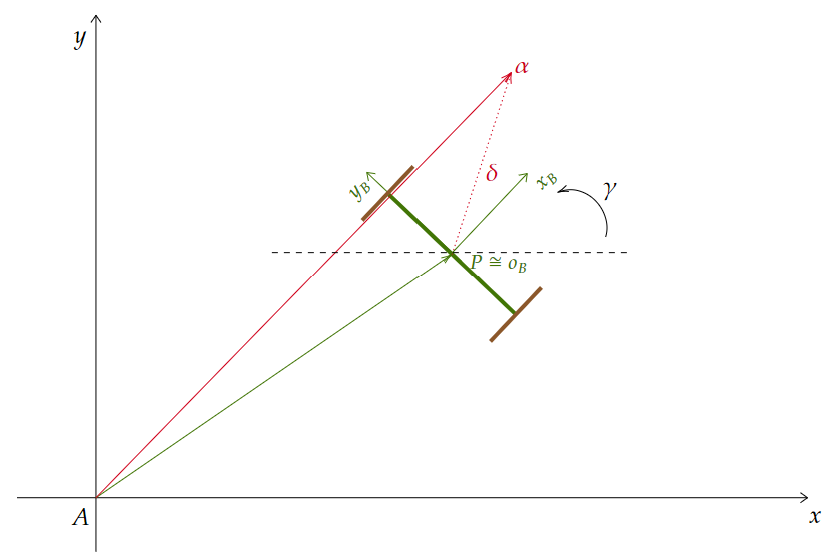
\includegraphics[width=0.7\linewidth]{unicycle singularity.png}
    \caption{Unicycle singularity.}
    \label{fig:Unicycle singularity}
\end{figure}


To address this undesirable behavior, our solution has been as follows: instead of controlling $P_x , P_y$, we control the $x-y$ position of a point ($\bm{\alpha}$) which is rigidly attached to the base, at a distance $\bm{\delta}$ from it, as shown in the image above. 

If we call A the world frame, the following relations can be written:

\begin{equation}
{}^{A} \bm{\alpha} = {}^{A}\mathbf{P} + {}^{A} R_{B} {}^{B} \bm{\delta}.
\label{eq:control point generic}
\end{equation}

This solution is enough for which concerns the tracking itself, but there is still something hidden in the robot dynamics, that makes the whole control problem unfeasible: when switching to the accelerations level (but this can also be directly observed from the position), the acceleration of this point becomes instantaneously linked to the pitch angular acceleration, making their coupled control complex.

This has been the reason why we kinematically defined a point which is still rigidly connected with the base reference frame $B$, but doesn't rotate with the base around the axis $y_B$ as described in Figure \ref{fig:accelerations decoupling}.
What changes between the two definitions is just the matrix ${}^{A}R_{B}$ which is no more the rotation matrix between frames $B$ and $A$, but become the matrix describing the \textit{elementary rotation} around the axis $z$, and we will call it ${}^{A}R^{xy}_{B}$

\begin{equation}
{}^{A} R_B^{xy} = \begin{bmatrix}
\cos(\psi) & -\sin(\psi) & 0 \\
\sin(\psi) & \cos(\psi) & 0 \\
0 & 0 & 1 \\
\end{bmatrix}. 
\end{equation}

\begin{figure}
    \centering
    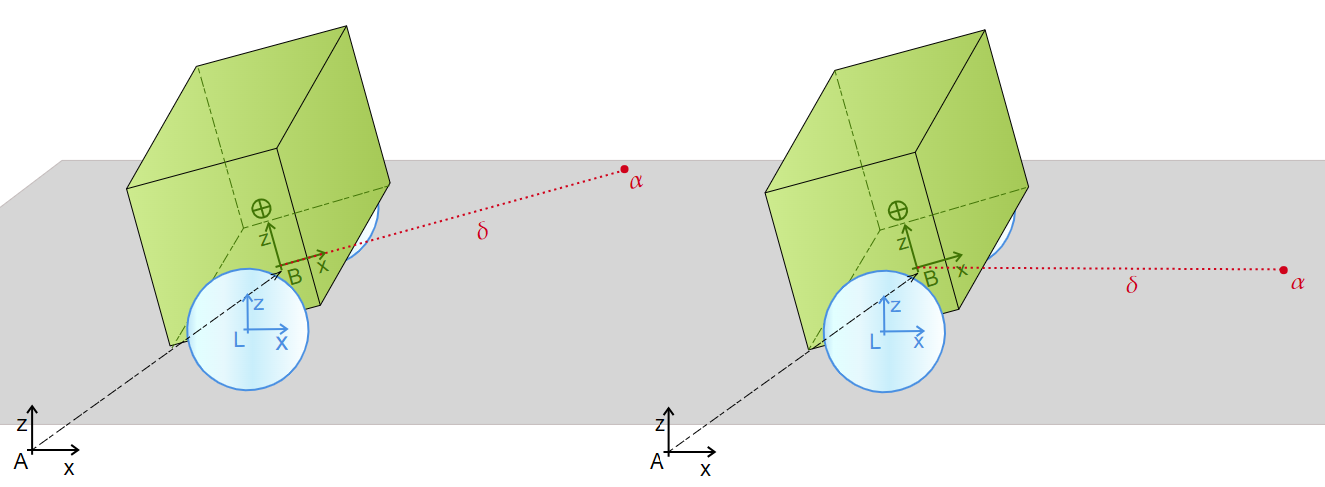
\includegraphics[width=0.85\linewidth]{accelerations decoupling.png}
    \caption{Accelerations decoupling.}
    \label{fig:accelerations decoupling}
\end{figure}

Also in this case we cannot directly impose a function of the robot configuration, but we have to derive twice the Equation \eqref{eq:control point generic} to end up in the control point acceleration.

The control point velocity is given by 

\begin{equation}
{}^{A} \dot{\bm{\alpha}} = \frac{d}{dt} ({}^{A} \bm{\alpha}) = {}^{A} \dot{\mathbf{P}} + {}^{A} \dot{R}_B^{xy} {}^{B} \bm{\delta}
\label{eq:control point velocity}
\end{equation}

and its acceleration is given by

\begin{equation}
{}^{A} \ddot{\bm{\alpha}} = \frac{d}{dt} ({}^{A} \bm{\dot{\alpha}}) = {}^{A} \ddot{\mathbf{P}} + {}^{A} \ddot{R}^{xy}_{B} {}^{B} \bm{\delta}
\label{eq:control point acceleration} 
\end{equation}

The complete derivation of the equation can be found in \cref{ch:Appendix}, here the final formulation of the control point acceleration is reported as affine function of the robot's generalized acceleration

\begin{equation}
\begin{aligned}
{}^{A} \ddot{\bm{\alpha}}_{xy} = & \; S_{v}J_{B}\dot{\bm{\nu}} - {}^{A} \dot{R}^{xy}_{B} ({}^{B}\bm{\delta}) ^\wedge S_{\omega}{}^{B}X_{B[A]}J_{B} \bm{\nu} \\
& - {}^{A} R^{xy}_{B}({}^{B}\bm{\delta})^\wedge S_{\omega}{}^{B} \dot{X}_{B[A]}J_{B} \bm{\nu} - {}^{A} R^{xy}_{B}({}^{B}\bm{\delta})^\wedge S_{\omega}{}^{B}X_{B[A]}J_{B} \dot{\bm{\nu}}.
\end{aligned}
\label{eq:control point acceleration affine}
\end{equation}

Also for this task, similarly to what has already been done in \cref{subsec:Self-Balancing Task} we have to define the error function to be minimized by the controller as stated in Equation \eqref{eq: Task equation with Jacobians}.

A simple manipulation of Equation \eqref{eq:control point acceleration affine}, defining the task Jacobian as

\begin{equation}
    J_{T_{\alpha}} = S_{v}J_{B} - {}^{A} R^{xy}_{B}({}^{B}\bm{\delta})^\wedge S_{\omega}{}^{B}X_{B[A]}J_{B}
    \label{eq: Tracking Task Jacobian}
\end{equation}

leads to 

\begin{equation*}
     \ddot{\bm{\alpha}}_{xy} = J_{T_{\alpha}}{\bm{\nu}} - J_{T_{\alpha}}\bm{\nu}.
\end{equation*}

Adopting the definition of desired acceleration provided in Equation \eqref{eq: Desired Acceleration}

\begin{equation}
    \ddot{\bm{\alpha}}_{xy}^{*} = \ddot{\bm{\alpha}}_{xy}^{n} -K_{d\alpha}(\dot{\bm{\alpha}}_{xy}-\dot{\bm{\alpha}}_{xy}^{n}) -K_{p\alpha}(\bm{\alpha}_{xy} - \bm{\alpha}_{xy}^{n})
    \label{eq: Alpha Desired Acceleration}
\end{equation}

where $K_{p\alpha}$ and $K_{d\alpha}$ are $2 \times 2$ diagonal matrices such as

\begin{equation}
    K_{p\alpha} = \begin{bmatrix}
        k_{p\alpha_x} & 0 \\
        0 & k_{p\alpha_y}
    \end{bmatrix}; K_{d\alpha} = \begin{bmatrix}
        k_{d\alpha_x} & 0 \\
        0 & k_{d\alpha_y}
    \end{bmatrix}.
\end{equation}

The final error function used for trajectory tracking control inside the TSID is 

\begin{equation}
   \mathbf{e(\bm{\alpha}_{xy},t)} =J_{T_{\alpha}}{\dot{\bm{\nu}}} - \dot{J}_{T_{\alpha}}\bm{\nu} - \ddot{\bm{\alpha}}_{xy}^{*} 
    \label{eq: Tracking error task}.
\end{equation}

\section{Constraints definition}
\label{sec:Constraints definition}

Once the tasks are defined, what is still missing is the formulation of the constraints. 
Our control problem requires three main constraints that are as follows:

\begin{itemize}
    \item Robot's dynamic equation
    \item Pure rolling contact constraint
    \item Forces friction cone constraint
\end{itemize}

The first has already been discussed in \cref{sec:E-Cargo Dynamical model}, while the others will be addressed in this section. 

\subsection{Pure Rolling Constraint}
\label{subsec:Pure Rolling Constraint}

We have seen in \cref{subsec:Constraints model} how a general rigid contact constraint is modeled.
Here the difference is that we cannot constrain the contact point to remain fixed for the whole contact duration, but we have to constrain its acceleration to be the desired one that guarantees rolling without slipping.

\begin{figure}
    \centering
    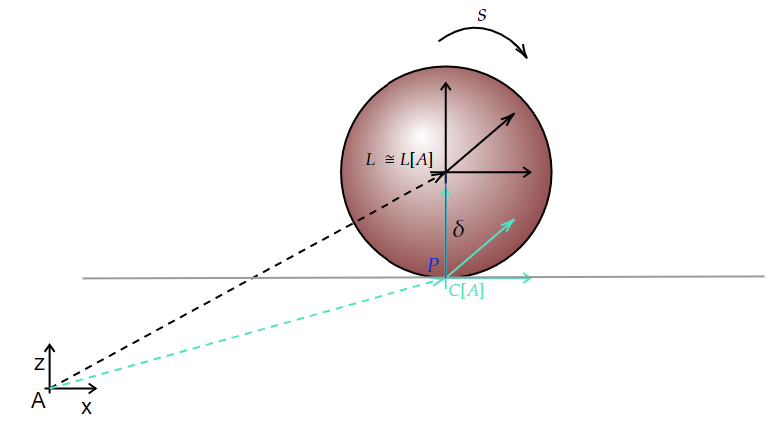
\includegraphics[width=0.65\linewidth]{Pure Rolling.png}
    \caption{Rolling kinematics.}
    \label{fig:Rolling kinematics}
\end{figure}

According to Figure \ref{fig:Rolling kinematics}, we define a generic point ${}^{A}\mathbf{P}_C$ that belongs to the circumference of the wheel and rotates together with the wheel's reference frame $L$

The point is kinematically defined as:

\begin{equation}
   {}^{A}\mathbf{P}_C = {}^{A} \mathbf{P}_{L} + {}^{A}R_{L} {}^{L}\bm{\delta} 
    \label{eq:Contact Point Position}
\end{equation}

and so its velocity is:

\begin{equation}
    {}^{A}\dot{\mathbf{P}}_{C} = {}^{A} \dot{\mathbf{P}}_{L} + {}^{A} \bm{\omega}^{\wedge{}}_{A,L} {}^{A}R_{L} {}^{L}\bm{\delta}. 
    \label{eq:Contact Point Velocity}
\end{equation}

Now, if we assume that at the instant considered, this point finds itself in the contact point between the wheel and the terrain, we can state that:

\begin{equation*}
    {}^{A}R_{L} {}^{L}\bm{\delta} = -r \mathbf{e_{3}}
\end{equation*}

where $r$ is the radius of the wheel.

If we substitute this equality inside the Equation \eqref{eq:Contact Point Velocity}, we can then impose the instantaneous velocity of a such defined point equal to zero to guarantee no slipping.

\begin{equation}
{}^{A}\dot{\mathbf{P}}_{C} = {}^{A} \dot{\mathbf{P}}_{L} - r {}^{A} \bm{\omega}^{\wedge{}}_{A,L} \mathbf{e_{3}} = 0.
\label{eq:Rolling velocity constraint}
\end{equation}

From this equation, we can obtain the expression for ${}^{A} \dot{\mathbf{P}}_{L}$, which is: 

\begin{equation}
{}^{A} \dot{\mathbf{P}}_{L} = r {}^{A} \bm{\omega}^{\wedge{}}_{A,L} \mathbf{e_{3}}.
\end{equation}

Deriving this expression, we end up in the constrain that we want to impose on the accelerations:

\begin{equation}
{}^{A} \ddot{\mathbf{P}}_{L} = r {}^{A} \dot{\bm{\omega}}^{\wedge{}}_{A,L} \mathbf{e_{3}}.
\end{equation}

And this relation is valid in mixed representation.

Also in this case the complete derivation of the equation can be found in \cref{ch:Appendix}, here just the final formulation of the contact point acceleration is reported as a function of the robot's generalized acceleration.

\begin{equation}
 (S_{v} J_{L} + r\mathbf{e_{3}}^{\wedge{}} S_{\omega} J_{L}) \dot{\bm{\nu}} + (r\mathbf{e_{3}}^{\wedge{}} S_{\omega} + S_{v}) \dot{J}_{L} \bm{\nu} = 0.
\label{eq: Pure Rolling Acceleration Constraint}
\end{equation}

At this point we group together some terms of Equation \eqref{eq: Pure Rolling Acceleration Constraint}, defining the constraint Jacobian as

\begin{equation}
    J_{R} = S_{v} J_{L} + r\mathbf{e_{3}}^{\wedge{}} S_{\omega} J_{L}.
    \label{eq: Rolling Jacobian}
\end{equation}

The final constraint formulation used inside the TSID is 

\begin{equation}
   \mathbf{c(\bm{q},t)} = J_{R}\bm{\dot{\nu}} + \dot{J}_R\bm{\nu} = 0.
    \label{eq: Rolling TSID contraint}
\end{equation}

\subsection{Forces Friction Cone}
\label{subsec:Forces Friction Cone}

We can sketch at this point a first version of the control problem, given the preliminary structure obtained by combining Equations \eqref{eq:e-Cargo dynamic equation} \eqref{eq: Pitch error task} \eqref{eq: Tracking error task} \eqref{eq: Rolling TSID contraint}.

\begin{center}
$\underset{\bm{\dot{\nu},{}_{B}\mathbf{f},\bm{\tau}}}{\text{argmin}} (W_{\alpha}\|J_{T_{\alpha}}{\dot{\bm{\nu}}} - \dot{J}_{T_{\alpha}}\bm{\nu} - \ddot{\bm{\alpha}}_{xy}^{*}\|^{2} + w_{\theta}\| J_{T_P}{\dot{\bm{\nu}}} - \dot{J}_{T_P}\bm{\nu} - \ddot{\theta}^{*} \|^{2})$

\text{subject to}

\end{center}

\begin{equation}
\begin{cases}
        M(\mathbf{q})\dot{\bm{\nu}} + C(\mathbf{q},\bm{\nu})\bm{\nu} + \mathbf{g}(\mathbf{q}) = S\bm{\tau} + J^{T}_{C} {}_{B}\mathbf{f} \\
        J_{R}\bm{\dot{\nu}} + \dot{J}_R\bm{\nu} = 0
\end{cases}
\label{eq: First TSID Structure}
\end{equation}

Notice that $W_{\alpha}$ is a diagonal matrix with task weights 

\begin{equation*}
    W_{\alpha} = \begin{bmatrix}
        w_{\alpha_x} & 0 \\
        0 & w_{\alpha_y}
    \end{bmatrix}.
\end{equation*}

There is still something missing:
In our control framework the contact forces are also optimization variables, but looking at Equations \eqref{eq: First TSID Structure}, at this level the controller is free to choose whatever values for the contact wrench ${}_{B}\mathbf{f}$ which respect the robot dynamic.
In real applications, we know that to ensure rolling without slipping, the forces have to lie inside the friction cone, which is generally defined as \cite{Pretorius-et-al}:

\begin{equation}
\begin{cases}
  f_z > f_z^{min} \geq 0\\
\\
 \sqrt{f_x ^{2} + f_y ^{2}} < \mu_c f_z \\
\end{cases}
\label{eq:nonlinear friction cone}
\end{equation}

where $\mu_c$ is the static friction coefficient and $f_x, f_y, f_z$ are respectively the $1^{st}, 2^{nd}, 3^{rd}$ components of a single 3D contact wrench.

The control problem we aim to set up is a Quadratic Program (QP), which can only accept affine constraints. Therefore, the friction cone is typically approximated by a generic polyhedron with an arbitrary number of sides ass shown in Figure (\ref{fig:Friction Cone Approximation}).

\begin{figure}
    \centering
    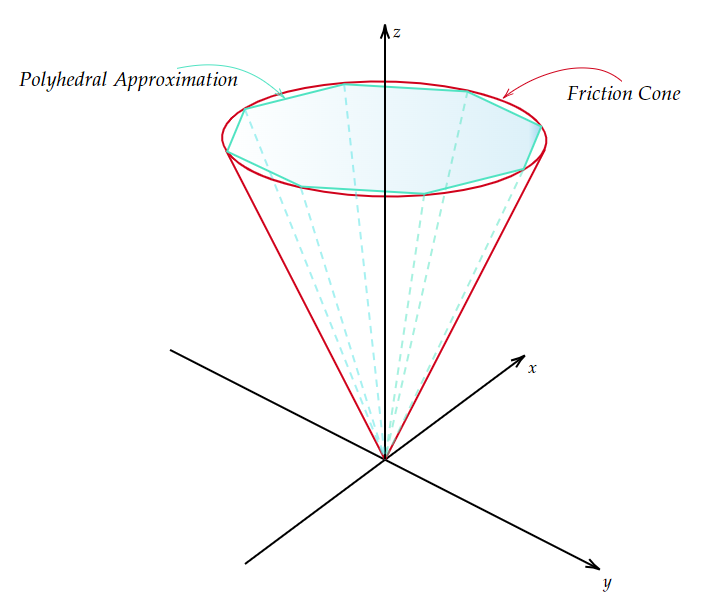
\includegraphics[width=0.5\linewidth]{Friction cone.png}
    \caption{Friction Cone Approximation.}
    \label{fig:Friction Cone Approximation}
\end{figure}

This approximation allows us to pass from the system of equations \eqref{eq:nonlinear friction cone}
to a matrix inequality like

\begin{equation}
    A_{f}{}_{B}\mathbf{f} < \mathbf{b}_{f}
\label{eq:Linear friction cone}
\end{equation}

where the size of the matrix $A_{f}$, and so the number of inequalities, depends on the number of the sides of the polyhedron; for our application in particular, we choose a polyhedron with eight sides.
Equation \eqref{eq:Linear friction cone} is then incorporated into the system in Equation \eqref{eq: First TSID Structure}.

\section{Nominal Trajectory Planner}
\label{sec:Nominal Trajectory Planner}

The version of the control problem in Equation \eqref{eq: First TSID Structure} with the addition of the inequality constraints in Equation \eqref{eq:Linear friction cone}, if properly tuned, could give some good results only if the performance requirements are low. 
This can be easily understood by examining the formulations of the desired accelerations in Equations \eqref{eq: Alpha Desired Acceleration} and \eqref{eq: Pitch Desired Acceleration}, which are written again here for clarity

\begin{equation*}
    \ddot{\bm{\alpha}}_{xy}^{*} = \ddot{\bm{\alpha}}_{xy}^{n} -K_d(\dot{\bm{\alpha}}_{xy}-\dot{\bm{\alpha}}_{xy}^{n}) -K_p(\bm{\alpha}_{xy} - \bm{\alpha}_{xy}^{n})
\end{equation*}

\begin{equation*}
    \ddot{\theta}^{*} = \ddot{\theta}^{n} -K_d(\dot{\theta}-\dot{\theta}^{n}) -K_p(\theta - \theta^{n})
\end{equation*}

The \textit{nominal trajectories} denoted with the apex $'n'$, are by definition feasible user defined trajectories that we want our robot to follow; this problem is dynamically coupled in the sense that the nominal trajectories that we want to impose for the stabilization ($\theta^{n}, \dot{\theta}^{n}, \ddot{\theta}^{n}$) have to be a function of the ones imposed or the tracking ($\bm{\alpha}_{xy}^{n}, \dot{\bm{\alpha}}_{xy}^{n}, \ddot{\bm{\alpha}}_{xy}^{n}$).

\begin{figure}
    \centering
    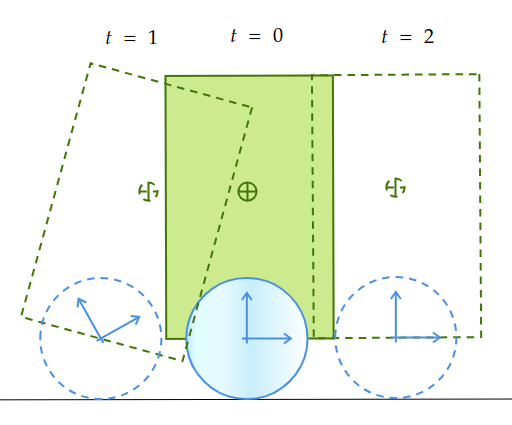
\includegraphics[width=0.6\linewidth]{nominal trajectory coupling.png}
    \caption{Nominal Trajectory Coupling.}
    \label{fig:Nominal Trajectory Coupling}
\end{figure}

With reference to Figure \ref{fig:Nominal Trajectory Coupling} we want to highlight that if the robot has to move on the right starting from an initial condition in which it is standstill with pitch angle $\theta =0$, it has to adjust the pitch angle according to the acceleration that we want on the rightward direction.
This means that if we do not define a proper relationship between the nominal trajectories, the controller will always attempt to minimize the largest error. However, every time the tracking error decreases, the stabilization error increases, and vice versa, leading to undesired oscillatory behavior that significantly reduces the achievable performances. 

This problem can be addressed in different ways that will be briefly discussed in \cref{ch:conclusions}, here we adopted a simple but effective solution: knowing that the goal is finding a relation of the type: $\theta^{n} = f (\ddot{\bm{\alpha}}_{xy}^{n}, t)$, we choose as $\theta^{n}$ the output of a PI controller on the in-plane velocity ($\dot{\alpha}_{x} + \dot{\alpha}_{y}$)

\begin{equation}
\theta^{n} =K_P((\dot{\alpha}_{x}^{n}+\dot{\alpha}_{y}^{n}) - (\dot{\alpha}_{x} + \dot{\alpha}_{y})) + K_I \int ((\dot{\alpha}_{x}^{n}+\dot{\alpha}_{y}^{n}) -(\dot{\alpha}_{x} + \dot{\alpha}_{y})) \  dt .
\label{eq:simple planner version}
\end{equation}

The PI controller in Equation \eqref{eq:simple planner version} acts as a linear nominal trajectory planner.
A simple block diagram of the entire control architecture is represented in Figure \ref{fig:TSID Control Block Diagram}

\begin{figure}
    \centering
    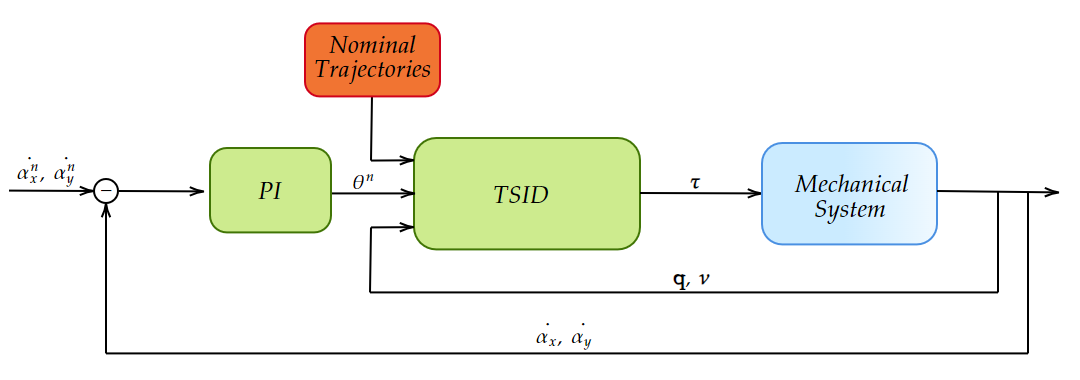
\includegraphics[width=1\linewidth]{Overall Scheme.png}
    \caption{TSID Control Block Diagram.}
    \label{fig:TSID Control Block Diagram}
\end{figure}


\section{Control Problem Formulation}
\label{sec:Control Problem Formulation}

The control problem now has all the elements and can be formulated in its complete version.

We first define the LSP formulation, and then pass to the more generic QP formulation.
\vspace{12pt}
\begin{center}
{\large \textbf{LSP Formulation}}
\end{center}

\begin{center}
$\underset{\bm{\dot{\nu},{}_{B}\mathbf{f},\bm{\tau}}, \bm{\xi}}{\text{argmin}} (W_{\alpha}\|J_{T_{\alpha}}{\dot{\bm{\nu}}} - \dot{J}_{T_{\alpha}}\bm{\nu} - \ddot{\bm{\alpha}}_{xy}^{*}\|^{2} + w_{\tau}\| \tau_L \|^{2} + w_{\tau}\| \tau_R \|^{2} + w_{\xi} \| \xi \|^{2} + {}_{B}\mathbf{f}^{T} \lambda I {}_{B}\mathbf{f})$

\text{subject to}

\end{center}

\begin{equation}
\begin{cases}
        M(\mathbf{q})\dot{\bm{\nu}} + h(\mathbf{q},\bm{\nu}) = S\bm{\tau} + J^{T}_{C} {}_{B}\mathbf{f} \\
        J_{R}\bm{\dot{\nu}} + \dot{J}_R\bm{\nu} = 0 \\
        J_{T_P}{\dot{\bm{\nu}}} - \dot{J}_{T_P}\bm{\nu} - \ddot{\theta}^{*} + \xi = 0 \\
        A_{f}{}_{B}\mathbf{f} < \mathbf{b}_{f} \\
        lb_{\xi} \leq \xi \leq ub_{\xi}
\end{cases}
\label{eq: LSP Formulation}
\end{equation}

With respect to the preliminary formulation given in Equation \eqref{eq: First TSID Structure}, some changes have been made

\begin{itemize}
    \item The stabilization problem involving the Equation \eqref{eq: Pitch error task} has been moved from the cost function to the constraints, with the addition of a slack variable $\xi$
    \item A double bounded inequality has been used to constrain the value of the slack variable $\xi$ which is then minimized inside the cost function as $w_{\xi} \| \xi \|^{2}$
    \item A \textit{regularization} term has been added on the contact forces with regularization coefficients $\lambda_{i}$ 
\end{itemize}

Since the Optimization-Based Control Problem is solved using a QP solver, the LS structure needs to be rearranged to conform to the conventional QP matrix formulation.
The complete derivation is performed in the \cref{ch:Appendix}, while here is reported just the final QP control structure


\vspace{12pt}
\begin{center}
{\large \textbf{QP Formulation}}
\end{center}

\begin{center}
$\underset{\bm{\dot{\nu},{}_{B}\mathbf{f},\bm{\tau}}, \bm{\xi}}{\text{argmin}} (\frac{1}{2} \mathbf{v}^{T} H \mathbf{v} + \mathbf{c}^{T} \mathbf{v})$
\text{subject to}
\end{center}

\begin{equation}
\begin{Bmatrix} 
-h(\mathbf{q},\bm{\nu})\\
-\dot{J_{R}}\bm{\nu} \\
\dot{J}_{T_P}\bm{\nu} + \ddot{\theta}^{*}\\
-\bm{\infty} \\
ub_{\xi} \\
\end{Bmatrix} \leq \begin{bmatrix} 
M(\mathbf{q}) & -J_c^{T} & -S & 0 \\
J_{R} & 0 & 0  & 0\\
J_{T_P} & 0 & 0  & 1\\
0 & A_{f} & 0 & 0\\
0 & 0 & 0 & 1 \\
\end{bmatrix} \begin{Bmatrix} 
\dot{\bm{\nu}} \\
{}_{B}\mathbf{f} \\
\bm{\tau}  \\
\xi \\
\end{Bmatrix} \leq \begin{Bmatrix} 
-h(\mathbf{q},\bm{\nu})\\\
-\dot{J_{R}}\bm{\nu}\\
\dot{J}_{T_P}\bm{\nu} + \ddot{\theta}^{*} \\
\mathbf{b}_{f} \\
ub_{\xi} \\
\end{Bmatrix}
\label{eq: QP Formulation}
\end{equation}